\documentclass[12pt,a4paper,oneside,english]{report}
\special{papersize=210mm,297mm}
%\usepackage[T1]{fontenc}
%\usepackage[latin1]{inputenc}
\usepackage[cm]{fullpage}
\usepackage[english]{babel}
\usepackage[pdftex]{graphicx}
\usepackage[labelsep=period]{caption}
\usepackage{subcaption}
\usepackage{color}
\usepackage{fixltx2e}
\usepackage{epstopdf}
\usepackage{hyperref}
\usepackage{gensymb}
\usepackage{float}
\usepackage{textcomp}
\usepackage{circuitikz}
%\usepackage{subfig}
\graphicspath{{./FIG}}

\begin{document}
\ctikzset{bipoles/length=.6cm}
\ctikzset{bipoles/thickness=4}
\newcommand\electricC {
\hspace{-14 pt}
\begin{circuitikz}
\draw (0,0) to[capacitor] (0:1);
\end{circuitikz}
\hspace{-6 pt}
}
\newcommand\electricR {
\hspace{-14 pt}
\begin{circuitikz}
\draw (0,0) to[european resistor] (0:1);
\end{circuitikz}
\hspace{-6 pt}
}
\newcommand\electricL {
\hspace{-14 pt}
\begin{circuitikz}
\draw (0,0) 
 to[american inductor] (-1,0) 
;\end{circuitikz}
\hspace{-6 pt}
}
\newcommand\electricDAK {
\begin{circuitikz}
\draw (0,0) to[full diode] (0:1);
\end{circuitikz}
}
\newcommand\electricDKA {
\begin{circuitikz}
\draw (0,0) to[full diode] (180:1);
\end{circuitikz}
}
\title{TransistorTester with AVR microcontroller \\
and a little more\\
Version 1.13k \\
}
\author{Karl-Heinz K\"ubbeler\\
\texttt{kh\_kuebbeler@web.de}}
\date{\today}
\maketitle
\tableofcontents

\include{00-preface}

%\newpage
\chapter{Features}
\label{sec:features}
\begin{enumerate}
\item Operates with ATmega8, ATmega168 or ATmega328 microcontrollers. Additionally ATmega644, ATmega1284,
ATmega1280 or ATmega2560 microcontrollers can be used.
\item Displaying the results to a 2x16 or a 4x16 character LCD-Display.
 If the processor have at least 32K flash memory, also a graphical display with 128x64 pixel and
a ST7565, ST7920, NT7108, KS0108 or a SSD1306 controller can be used.
In doing so a 4-wire SPI interface or a I\textsuperscript{2}C bus must be used instead of the 4-bit parallel interface for
the SSD1306 controller.
Even color displays with ILI9163 or ST7735 controller are usable with the SPI interface.
For the NT7108 or KS0108 controller you must use a serial - parallel interface with a 74HC(T)164 or a 74HC(T)595.
Displays with PCF8812 or PCF8814 controller can be only used without the big icons for transistors, because the display size is
unsufficient (102x65 and 96x65).
\item One key operation with automatic power shutdown.
\item Battery operation is possible since shutdown current is only about \(20nA\).
\item Low cost version is feasible without crystal and auto power off.
With software version 1.05k the sleep modus of the Atmega is used to reduce current if
no measurement is required and no rotary encoder is used (not with ATmega8).
\item Automatic detection of NPN and PNP bipolar transistors, N- and P-Channel MOSFETs, JFETs,
diodes, double diodes,N- and P-IGBTs, Thyristors and Triacs.
For Thyristors and Triacs the ignition current and holding current must be reached with the tester.
For IGBTs the \(5V\) signal should be enough for driving the gate voltage.
\item Automatic detection of pin layout of the detected part.
\item Measuring of current amplification factor and Base-Emitter threshold voltage of bipolar transistors.
\item Darlington transistors can be identified by the threshold voltage and high current amplification factor.
\item Detection of the protection diode of bipolar transistors and MOSFETs.
\item Measuring of the Gate threshold voltage, the Gate capacity value and the R\textsubscript{DSon} at almost \(5V\) gate voltage of MOSFETs.
\item Up to two Resistors are measured and shown with symbols
\begin{circuitikz}
\draw (0,0) to[european resistor] (0:1);
\end{circuitikz}
and values with up to four decimal digits in the right dimension.
All symbols are surrounded by the probe numbers of the Tester (1-3).
So Potentiometer can also be measured. If the Potentiometer is adjusted to one of its ends,
the Tester cannot differ the middle pin and the end pin.
\item Resolution of resistor measurement is now up to \(0.01\Omega\), values up to \(50M\Omega\) are detected.
\item One capacitor can be detected and measured. It is shown with symbol
\begin{circuitikz}
\draw (0,0) to[capacitor] (0:1);
\end{circuitikz}
and value with up to four decimal digits in the right dimension. 
The value can be from \(25pF\) (\(8MHz\) clock, \(50pF\) @\(1MHz\) clock) to \(100mF\). The resolution can be up to \(1pF\) (@\(8MHz\) clock].
\item For capacitors with a capacity value above \(20nF\) the Equivalent Serial Resistance (ESR) is measured 
with a resolution of \(0.01\Omega\) and is shown with two significant decimal digits.
This feature is only available for ATmega with at least 16K flash memory.
\item For capacitors with a capacity value above \(5000pF\) the voltage loss after a load pulse can be determined.
The voltage loss give a hint for the quality factor of the capacitor.
\item Up to two diodes are shown with symbol
\begin{circuitikz}
\draw (0,0) to[full diode] (0:1);
\end{circuitikz}
or symbol
\begin{circuitikz}
\draw (0,0) to[full diode] (180:1);
\end{circuitikz}
in correct order. Additionally the flux voltages are shown.
\item LED is detected as diode, the flux voltage is much higher than normal. 
Two-in-one LEDs are also detected as two diodes.
\item Zener-Diodes can be detected, if reverse break down Voltage is below \(4.5V\).
These are shown as two diodes, you can identify this part only by the voltages.
The outer probe numbers, which surround the diode symbols, are identical in this case.
You can identify the real Anode of the diode only by the one with break down (threshold) Voltage nearby \(700mV\)!
\item If more than 3 diode type parts are detected, the number of founded diodes is shown additionally to the fail message.
 This can only happen, if Diodes are attached to all three probes and at least one is a Z-Diode.
In this case you should only connect two probes and start measurement again, one after the other.
\item Measurement of the capacity value of a single diode in reverse direction.
Bipolar Transistors can also be analysed, if you connect the Base and only one of Collector or Emitter.
If a ATmega with more than 8K flash memory is used, also the reverse current of the diode is measured with
a resolution of \(2nA\).
The value is only output to the screen, if it is greater than zero.
\item Only one measurement is needed to find out the connections of a bridge rectifier.
\item Capacitors with value below \(25pF\) are usually not detectet, but can be measured together with
a parallel diode or a parallel capacitor with at least \(25pF\).
In this case you must subtract the capacity value of the parallel connected part.
For processors with at least 32K flash memory the tester changeover to a special capacity meter function,
if a capacitor with more than \(25pF\) is once measured at TP1 and TP3. In this capacitor meter mode you
can measure capacitors below \(25pF\) at TP1 and TP3 directly.
\item For resistors below \(2100\Omega\) also the measurement of inductance will be done, if
your ATmega has at least 16K flash memory.
For that a inductor icon
\begin{circuitikz}
\draw (0,0) to[american inductor] (180:1);
\end{circuitikz}
is shown behind the resistor icon
\begin{circuitikz}
\draw (0,0) to[european resistor] (0:1);
\end{circuitikz}
.
The range will be from about \(0.01mH\) to more than \(20H\), but the accuracy is not good.
The measurement result is only shown with a single component connected.
\item Testing time is about two seconds, only capacity or inductance measurement can cause longer period.
\item Software can be configured to enable series of measurements before power will be shut down.
\item Build in selftest function with optional \(50Hz\) Frequency generator to check the accuracy of clock frequency and wait calls (only for processors with at least 32K flash memory).
\item Selectable facility to calibrate the internal port resistance of port output and
the zero offset of capacity measurement with the selftest (only for processors with at least 16K flash memory).
A external capacitor with a value between \(100nF\) 
and \(20\mu F\) connected to pin~1 and pin~3 is necessary to compensate the offset voltage of the analog comparator.
This can reduce measurement errors of capacitors of up to \(40\mu F\).
With the same capacitor a correction voltage to the internal reference voltage is found to adjust the
gain for ADC measuring with the internal reference.
\item Display the Collector cutoff current \(I_{CE0}\) with currentless base (\(1\mu A\) units) and
Collector residual current \(I_{CES}\) with base hold to emitter level (only for processors with at least 16K flash).
This values are only shown, if they are not zero (especially for Germanium transistors).
\item For a ATmega with at least 32K flash memory the tester changes the operation modus from universal tester
to a resistor tester, if only one resistor is detected at the test pin 1 (TP1) and test pin 3 (TP3).
If you have selected the additional measurement of inductance for the resistor meter function with the 
Makefile option RMETER\_WITH\_L, also the inductance of components is measured in this mode.
This special operating mode is indicated with a [R] or [RL] at the right side of the first display line.
In the same way the tester changes to a capacity meter function, if a capacitor is detected at TP1 and TP3.
This operation mode is indicated with a [C] at the right side of the first display line.
With this capacity meter function capacity values are shown down to \(1pF\). Only for the automatic
start you need a capacitor with more than \(25pF\).
Both special modes can be finished by a key press. 
The tester will then continue with the normal tester function.
\item For processors with at least 32K flash a dialog function can be selected, which enable additional functions.
Of course you can return from dialog to the normal Transistor Tester function.
\item With dialog function you can use a frequency measurement at port PD4 of the ATmega.
The resolution is \(1Hz\) for input frequencies above \(33kHz\).
For lower frequencies the resolution can be up to \(0.001mHz\) by measuring the mean period.
You should read the the subsection Frequency measurement \ref{sec:frequency_counter} at page \pageref{sec:frequency_counter} 
for details of connection a frequency signal.
\item With the dialog function and without the activated serial output a external voltage of up to \(50V\) can be measured with
the 10:1 voltage divider at the PC3 port. If the PLCC-Version of the ATmega328 is used, one of the additional
pins can be used for the voltage measurement together with the serial output.
If the zener diode measurement extension (DC-DC converter) is assembled, the measurement of
zener diodes is also possible with this function by pressing the key.
\item With the dialog function a frequency output can be selected at the TP2 pin (PB2 Port of the ATmega).
Currently frequencies from \(1Hz\) up to \(2MHz\) can be selected.
\item With the dialog function a fixed frequency output with selectable pulse width can be activated at the TP2 pin
(PB2 port of the ATmega). The width can be enhanced with \(1\%\) by a short key press or with \(10\%\) by a longer key press.
\item With the dialog function can be started a separated capacity measurement with ESR measurement.
Capacities from about \(2\mu F\) up to \(50mF\) can most be measured in circuit, because only a little
measurement voltage of about \(300mV\) is used.
\item If your ATmega has at least 32K flash memory (Mega328), you can also use the sampling method of the ADC,
which can measure capacitors with less than 100pF at a resolution of up to 0.01pF.
With the same method you can also measure coils with less than 2mH with significant better resolution of the inductance
by building a resonant circuit with a parallel capacitor of known capacity value.

\end{enumerate}

You should make sure, that all capacitors have no residual charge before starting any measurement,
especially if you use the tester for measurement of capacitor in circuit.


Thyristors and Triacs can only be detected, if the test current is above the holding current.
Some Thyristors and Triacs need as higher gate trigger current, than this Tester can deliver.
The available testing current is only about \(6mA\)!
Also a IGBT can only be detected correctly, if a voltage of \(5V\) is sufficient to drive the gate.
Notice that many features can only be used with microcontroller with enough program memory such as ATmega168.
Only processors with at least 32k flash memory like ATmega328 or ATmega1284 can take all features.

\vspace{1cm}
\textbf{{\Large Attention:}} Allways be sure to {\bf discharge capacitors} before connecting them to the Tester!
The Tester may be damaged before you have switched it on. There is only a little protection at the ATmega ports.

Extra causion is required if you try to test components mounted in a circuit.
In either case the equipment should be disconnected from power source and you should be sure,
that {\bf no residual voltage} remains in the equipment.



\include{20-hardware}

\include{30-manual}

\include{40-configuring}

\include{50-measurement}

 \include{51-semicon}
 \include{52-resistors}
 \include{53-capacitors}
 \include{54-inductors}
 \include{55-selftest}
 
%\newpage
\section{��������� �������}
\label{sec:frequency}

������� � ������ 1.10k � ���� �������������� ������� ����� ������� ����� �Frequency� (��������� �������). 
����������� ��������� ������� �������������� ��������� ���������� ������ ������� �������� ������� �� ����� 
T0 (PD4) �� ���� �������. ��� ��������� ������� ����� � 1 ������� ������� 1 ������������ � 
������������� 256:1 ������� ����������.  
��� ��������� 1 ���������� ��������� �� ���� ������ ����� ������������ 16 ��������� ������� ATmega 
� �������� ���������� \(16~MHz\) � � �������������.
��� ������� � ��������� �������� 0 ������������ �������� ��������� B � A �������� 1. ����� �������� 
������ �������� ��� ������ ���������� ��������� �������� �������, ������������ ����������� ���������� 
������� ������� � ��������� �������� 1. ������� �������� � ����� ������������� ������������ ���������� 
����������� �����. ��� ����������� �������� ������� 1 ������� ���������� �������� �������������. 
��� ������� �� ����������, ������� �� ������� ����� ���� ���������������.\\

��� ������ ���� \(25~kHz\) ���������� ����������� ��������� � ����������� ���������� ������� �������. 
��� �������������� ��������� ������� ������ ����� ������������ ��������� �������. ��������� ������� 
����� ������� ����� �������� ���������� ���������� �� ����� PCINT20 (PD4) ��������� 0.
��� ��������� ������� �������� ������ ��� ��������������, ��� � �������������� ������������, 
������ ���� �� ����� \(10~\mu s\).  
������� 0 ������������ �� ������������ �������� �������. ���������� ����������  \(125~ns\) ���
\(8~MHz\). ��� ���������� �������� �������� ��������� ���������� ����� ���� ���������. 
��� ������������� 125 �������� ���������, ������� ���������� ��� ������ ������� �������� \(1~ns\). 
��� �������������� ���������� ������� � ��������� �������� 0, ������ �����
���������� �� �������, � ������� �� ���������� ��������� �� �������� ���������� PCINT20 �� ��� �� 
����� ��������� ������������ ����������. ���������� �������� ������� ���, ����� ����� ���� �������� 
����� ����� 10 ��������� ������ ������� ����������. ��� ����� ������ ������ �������� 
����� \(0,1~ppm\). � �������� �������� \(8~MHz\) ����� ��������� ���������� ����� 1,25 �������. 
��� ������������, ����� �������, ������� �������� �������, ������� ����������� 
����� � ����� ������� �����������.\\

��������� �������� ��������� ���: ��� ������� �������� ���� �����. ������ ����: ������� ������������ 
�������� 2 � ���������� �������� 1. ����� ����� ������� �������� �������, � ��������� �����������. 
�� ������� \ref{fig:freq-ppm} ������������ ���������� ����� ����� ���������. ����� ���������� 
���������� ����� ��������� ��������� �������� ������ ���� �������.

\begin{figure}[H]
\centering
\input{../GNU/frequency-ppm}
\caption{������������� ����������� ��������� �������}
\label{fig:freq-ppm}
\end{figure}

\subsection{���������� ������� �� GPS- ��� GLONASS-���������}

���������� ������� ������ ����� ����������� ��������� ������������ ������������ (\(5-25~pF\)).
������� �������������� ���������� ������� ������ ������� ���������� 1PPS � ����������� GPS ��������� 
{\bf UP501} �� {\bf Fastrax Ltd.} ��� � �������������� GPS/GLONASS ��������� {\bf GNS701} �� {\bf Global 
Navigation Systems GmbH}.
���������� ������ ����� ����� ��������� �� \(1000,000~ms\).
������ ��������� ����� ����� ���������� �� �������.
�������, ������� ��������� ������� �� �����������. ������� �� �� ������ ������� ����� ������� ������������ 
������ �����.

�� ������� \ref{fig:GPS-1PPS} ��������� ����� ����������� UM232 USB-����������������� ����������� �
��������� � ����������.

��������� UM232 ������������� ������������ ��� ���������� \(5~V\) � \(3,3~V\) 
��� ������� ����� �� USB. 

��� ������ ��������� ����������� � ���������� �� �����������. 
������ ������� 5~V ���������� ������ USB �����������. 

\begin{figure}[H]
  \begin{subfigure}[b]{9cm}
    \centering
    \includegraphics[width=8.5cm]{../FIG/GPS_UP501.eps}
    \caption{GPS}
  \end{subfigure}
  ~
  \begin{subfigure}[b]{9cm}
    \centering
    \includegraphics[width=8.5cm]{../FIG/GPS_GNS701.eps}
    \caption{GPS/GLONASS}
  \end{subfigure}
  \caption{��������� 1PPS ������� �� GPS ���������}
  \label{fig:GPS-1PPS}
\end{figure}

\subsection{���������� ������� � ������� ��������� ������}

����� ��������� ������� ��������� �������������� �������, �� ������ ������� �������� ���� ��
������������� � ������� ������ �� �������. ������������ ������������� ������� RTC ��� ����������
������� ������ ������� GPS ��� GLONASS ����������� � ���, ��� ��� �� ����� ���������� � ����
��������� ��������.
�� ������ ��������� ������� ����� � ����� �����.
� ���������� ������ ����� � ����� DS3231 � �������� ������ � �ZS-042�.
������������� ������, ��������, ������������ � �����, � ��� ����� �������� ����� DS3231M.
���������� DS3231M ���������� ��������� MEMS (Micro Electro Mechanical System) ������
���� DS3231SN, ������� ���������� �������� � \(32~768~Hz\).
���������������� ��������� MEMS ����� ������������ ����� DCP1301.
�� �������~\ref{fig:DS3231M} ������� ���� �� ������������ �������.

\begin{figure}[H]
\centering
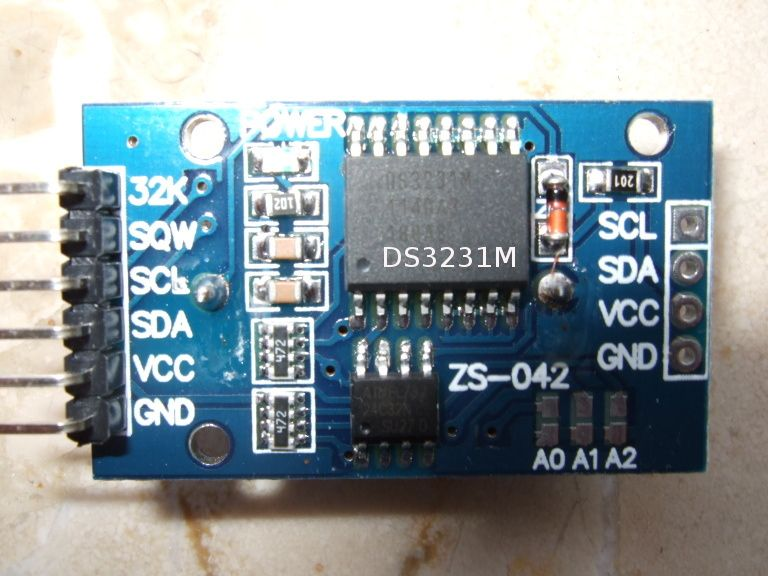
\includegraphics[width=9cm]{../PNG/DS3231M.jpg}
\caption{���� �� ���������������� DS3231 �������}
\label{fig:DS3231M}
\end{figure}

��� ������ ����� DS3231 ���������� ���������� ��������� ����������� ��� ���������� ������� ��������
����� �������, ��� ����� ������� � ������� ��������� ��� ��������� ����������� ����� ��������� ��������������.
� ���������, ��������������� ������ \(32~kHz\) ��� ���� DS3231M �� ����� �������������� ��� ����������
�������. ��� ��������� � ������� ������ �������: \(32~641~Hz\), \(32~710~Hz\), \(32~730~Hz\) � \(32~748~Hz\) ��� ���� 
������� ����������� �������.
��� ��� ������� ��������� ������ �� ��������� ������ ������� \(32~768~Hz\).
���� �� ����������� ������ � Arduino UNO, �� ����� ������ ������������ ����� 1PPS (\(1~Hz\)) � ������ SQW.
���� ����� ��������� �������� � ������, ��� ��� ����� ������������ ��� ����������.
������� DS3231M ������� ��� 1PPS ������ �������� \(pm 5~ppm \) ��� ������� ��������������
��������� �� \(-45\celsius\) �� \(+85\celsius\), � �������� \(32~kHz\) �� ������
��������������� ������ \(\pm 2.5\%\) (\(25000 ppm\)).

���� ������ ���� DS3231SN ������� �������� \(pm 3,5ppm\) ��� ������� ��������� ����������
�� \(-40\celsius\) �� \(+85\celsius\) � �������� \(\pm 2ppm\) ��� ����������� ����� \(0\celsius\)
� \(+40\celsius\). � ���� DS3231SN ������������ ���������� �������� �������� � �������� \(32~768~Hz\),
������� �������� ��������������� �������������� �������������� � ������� ������������� ���������.
��� ��������� ������������� ������ ��������� � ��������� ����������� ������� ��������������� ��������� �����
���������.
����� ��������� ��� ����, � ������� ���� DS3231M ������ DS3231DS ��� ���� ������� �������.

� ��������������� ������������� �������� (������ \(16~MHz\)) � ������� �������� ������� ���� �������
� ����� � ��� �� ����������� \(32,76800~kHz\). �� ����� ���������, ����� �����, �����������
������� � \(0,03~Hz\). ��� ������� ���������� ������ \(1ppm\).
������� ���������� \(1~Hz\) ������������ ������, ���� ������� ����������� ��� ��������� �������.
������ ��� ��������� ������� ������� � \(25~kHz\) �� \(33~kHz\), ����� ������� ��������� �������
��� ������� \(32~768~Hz\) ����� ������.



\include{60-generators}
\include{70-errors}
\include{80-special}
\include{90-todo}

\begin{thebibliography}{99}

\bibitem{Frejek}
Markus Frejek
\emph{AVR-Transistortester,}.
Embedded Projects Journal,
11. Ausgabe,
2011

\bibitem{ATmega8}
Atmel Corporation
\emph{8-bit AVR with 8KBytes In-System Programmable Flash - ATmega8(L),}.
Manual,
2486Z-AVR-02/11,
2011

\bibitem{ATmega168}
Atmel Corporation
\emph{8-bit AVR with 4/8/16/32KBytes In-System Programmable Flash - ATmega48 - ATmega328,}.
Manual,
8271D-AVR-05/11,
2011

\bibitem{AVR126}
Atmel Corporation
\emph{Atmel AVR126: ADC of megaAVR in Single Ended Mode,}.
Application Note,
8444A-AVR-10/11,
2011

\bibitem{AVR121}
Atmel Corporation
\emph{Atmel AVR121: Enhancing ADC resolution by oversampling,}.
Application Note,
8003A-AVR-09/05,
2005

\bibitem{LaTeX}
\url{http://en.wikibooks.org/wiki/LaTeX}
\emph{LaTeX documentation,}.
Guide to the LaTeX markup language,
2012

\bibitem{Gnuplot}
\url{http://en.wikibooks.org/wiki/Gnuplot}
\emph{Gnuplot documentation,}.
Documentation for the plotting tool gnuplot,
2012

\bibitem{ESR}
Wikipedia
\url{http://de.wikipedia.org/wiki/Equivalent\_Series\_Resistance}
\emph{Explanation for ESR in german language}.
Standardization and equivalent circuit of a capacitor,
2012


\bibitem{Xfig}
\url{http://www.xfig.org/userman}
\emph{Xfig documentation,}.
Documentation of the interactive drawing tool xfig,
2009

\bibitem{gimp}
\url{http://docs.gimp.org/2.6/de}
\emph{gimp documentation}.
Documentation of the GNU Image Manipolation Program,
2010

\bibitem{markus1}
\url{http://www.mikrocontroller.net/articles/AVR-Transistortester}
\emph{Online documentation of the Transistortester,}
Online Article,
2009-2011

\bibitem{avrdude}
\url{http://www.mikrocontroller.net/articles/AVRDUDE}
\emph{Online documentation of avrdude programmer interface,}
Online Article,
2004-2011

\bibitem{markus2}
\url{http://www.mikrocontroller.net/topic/131804}
\emph{Thread from Markus,}
Forum thread, 
2009

\bibitem{karlheinz1}
\url{http://www.mikrocontroller.net/articles/AVR\_Transistortester}
\emph{Short description of new features of the TransistorTester von Karl-Heinz K.,}
Online Article,
2012

\bibitem{karlheinz2}
\url{http://www.mikrocontroller.net/topic/248078}
\emph{Thread from Karl-Heinz,}
Thread and new software versions,
2012

\bibitem{winavr1}
\url{http://www.mikrocontroller.net/articles/WinAVR}
\emph{Information about WinAVR in german language,}
Online Article,
2012

\bibitem{winavr2}
\url{http://sourceforge.net/projects/winavr/files}
\emph{Source for WinAVR package,}
Download source,
2012

\bibitem{winavr3}
\url{http://www.mikrocontroller.net/topic/248078?page=5#2922341}
\emph{Patch for WinAVR, Setting of Fuses with avrdude,}
Download source,
2012

\bibitem{st7565}
\url{http://www.orientdisplay.com/pdf/ST7565.pdf}
\emph{Datasheet of the ST7565 graphical controller,}
Download source,
2014

\bibitem{ds3231}
Maxim Integrated Products, Inc.
\url{http://maximintegrated.com}
\emph{DS3231: Extremely Accurate I\textsuperscript{2}C-Integrated RTC/TCXO/Crystal,}
Data Sheet,
19-5170;Rev 10; 3/15,
2015

\bibitem{ds3231m}
Maxim Integrated Products, Inc.
\url{http://maximintegrated.com}
\emph{DS3231M: 5ppm I\textsuperscript{2}C Real-Time Clock,}
Data Sheet,
19-5312;Rev 7; 3/15,
2015



\end{thebibliography}
\end{document}

